\section{Project Support}
\label{sec:fdsp-coord-supp}

As defined in the \dword{dune} Management Plan (DMP), the \dword{dune}
Technical Board (TB) generates and recommends technical decisions to the 
collaboration executive board (EB) (see Fig.~\ref{fig:TB_org}).
\begin{figure}[htb]
  \begin{center}
    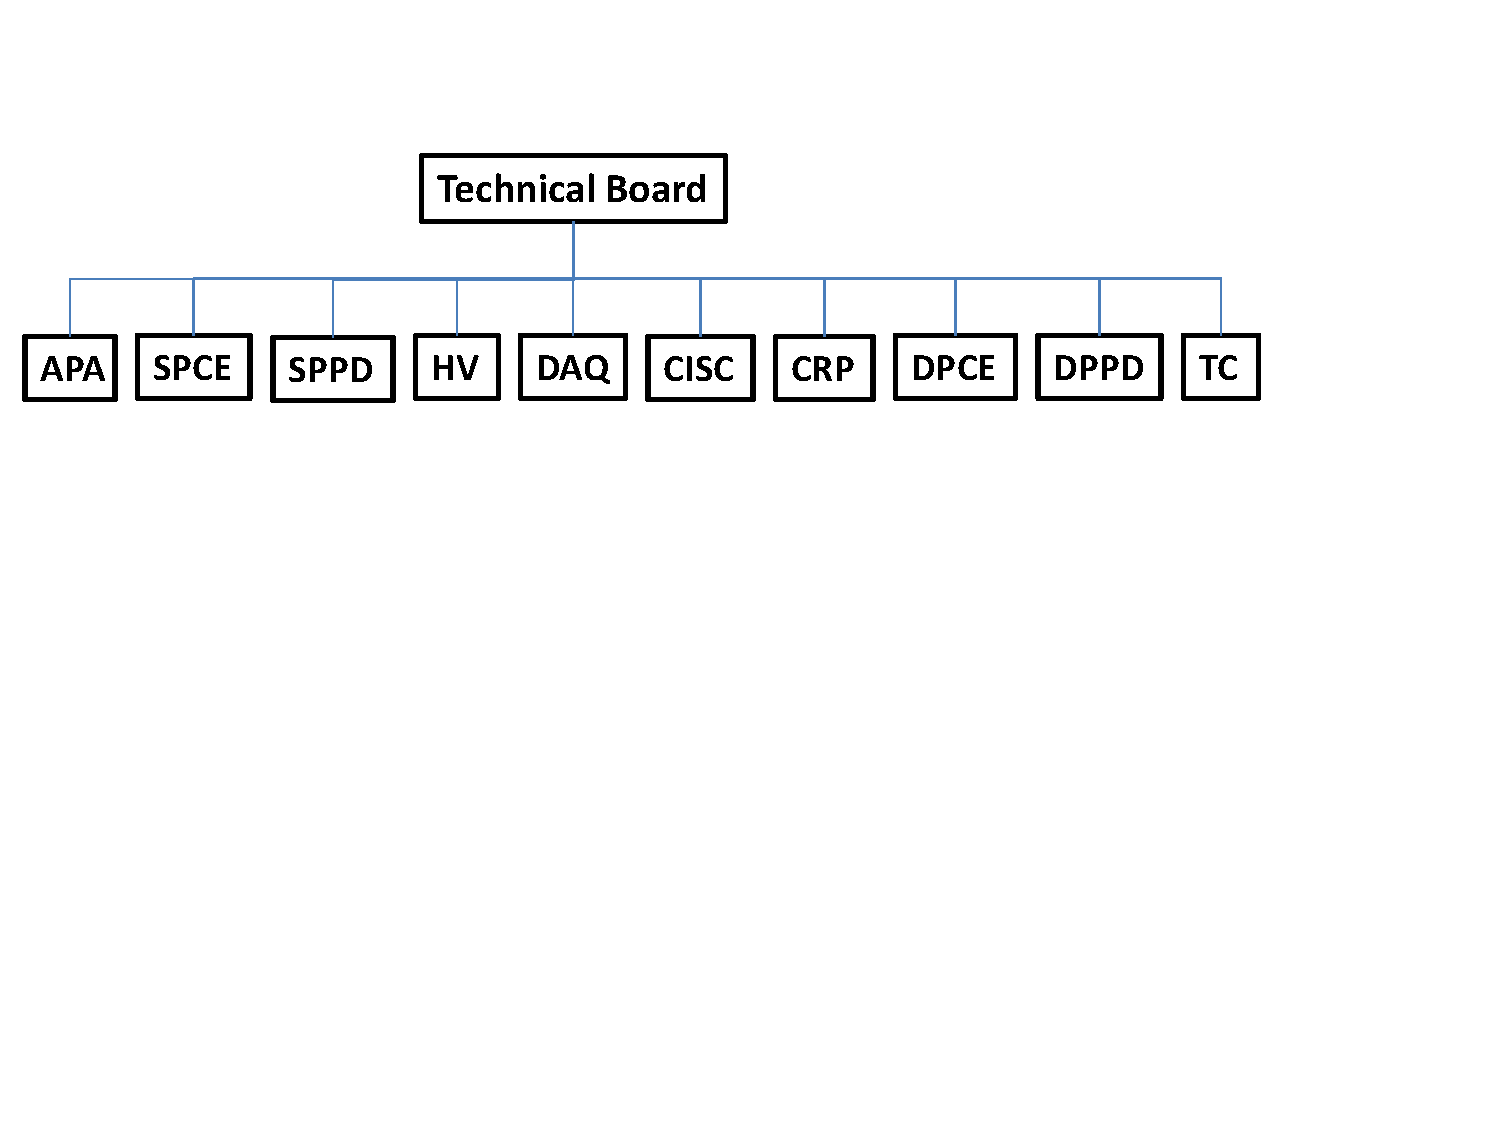
\includegraphics[width=\textwidth]{far-detector-generic/figures/TB_Org_Chart}
    \caption{DUNE Technical Board.}
    \label{fig:TB_org}
  \end{center}
\end{figure}
It consists of all consortia scientific and technical leads. It meets
on a regular basis (approximately monthly) to review and resolve any
technical issues associated with the detector construction. It reports
through the EB to Collaboration Management. The \dword{dune} TB
is chaired by the Technical Coordinator. DUNE collaboration
management, including the EB, is shown in Fig.~\ref{fig:DUNE_org}. The
\dword{tc} engineering team also meets on a regular (approximately monthly)
basis to discuss more detailed technical issues. \dword{tc} does not have
responsibility for financial issues that will instead be referred to
the EB and Resource Coordinator (RC).
\begin{figure}[htb]
  \begin{center}
    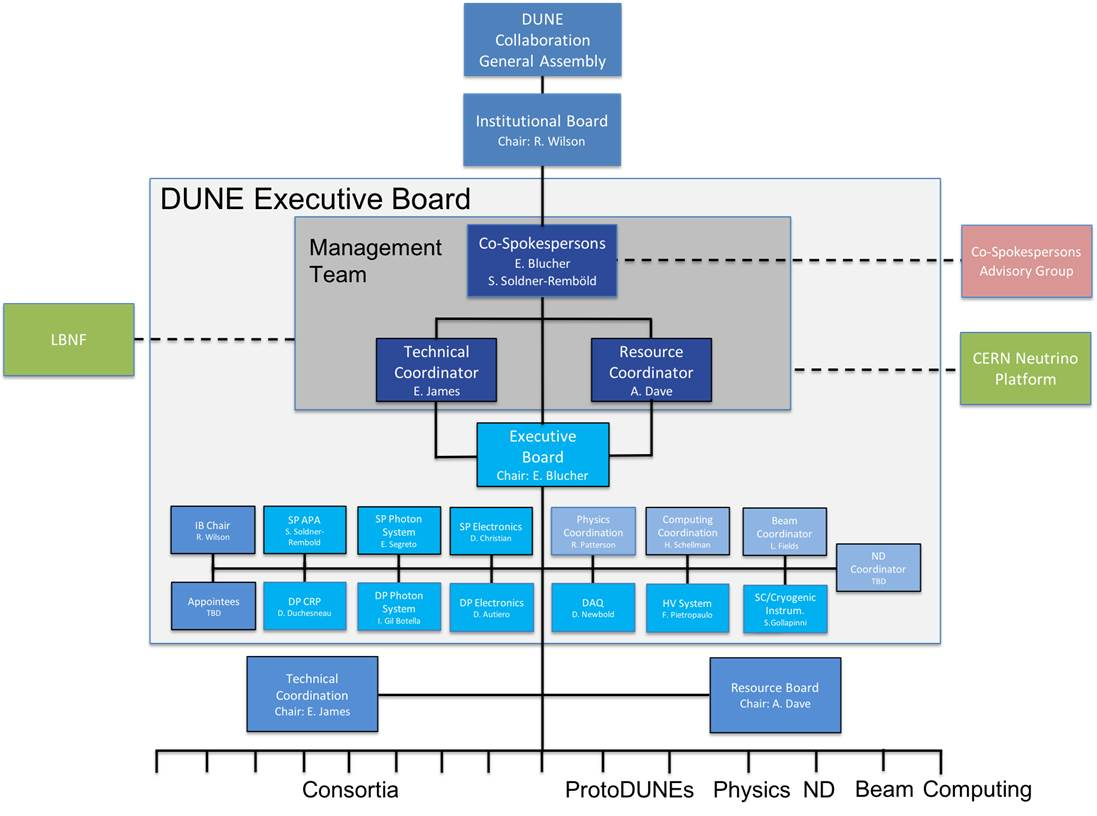
\includegraphics[width=\textwidth]{far-detector-generic/figures/DUNE_mgmt}
    \caption{DUNE management organizational structure.}
    \label{fig:DUNE_org}
  \end{center}
\end{figure}



\dword{tc} has several major project support tasks that need to be accomplished:
\begin{itemize}
  \item Assure that each consortium has a well defined and complete
    scope, that the interfaces between the consortia are sufficiently
    well defined and that any remaining scope can be covered by \dword{tc}
    through Common Fund or flag as missing scope to the EB and RC. In
    other words to assure that the full detector scope is
    identified. Monitor the interfaces and consortia progress in
    delivering their scope.
  \item Develop an overall project integrated master schedule (IMS)
    that includes reasonable production schedules, testing plans and a
    well developed installation schedule from each consortia. Monitor
    the IMS as well as the individual consortia schedules.
  \item Ensure that appropriate engineering and safety standards are
    developed and agreed to by all key stakeholders and that these
    standards are conveyed to and understood by each
    consortium. Monitor the design and engineering work.
  \item Ensure that all \dword{dune} requirements on \dword{lbnf} for
    conventional facilities, cryostat and cryogenics have been clearly
    defined and understood by each consortia. Negotiate scope
    boundaries with \dword{lbnf}. Monitor \dword{lbnf} progress on
    final conventional facility design, cryostat design and cryogenics
    design.
  \item Ensure that all technical issues associated with scaling from
    \dword{protodune} have sufficient resources to converge on
    decisions that enable the detector to be fully integrated and
    installed.
  \item Ensure that the integration and QC processes for each
    consortia are fully developed and reviewed and that the
    requirements on an \dword{itf} are well defined.
\end{itemize}

\dword{tc} is responsible for technical quality and schedule and is not
responsible for consortia funding or budgets.  \dword{tc} will try to help
resolve any issue that it can, but will likely have to push all
financial issues to the TB, EB and RC for resolution.

\dword{tc} maintains a web page
(\url{https://web.fnal.gov/collaboration/DUNE/DUNE\%20Project/\_layouts/15/start.aspx\#/})
with links to project documents. \dword{tc} maintains repositories of project
documents and drawings. These include the WBS, schedule, risk
register, requirements, milestones, strategy, detector models and
drawings that define the \dword{dune} detector.


%%%%%%%%%%%%%%%%%%%%%%%%%%%%%%%%
\subsection{Schedule}
\label{sec:fdsp-coord-controls}

A series of tiered milestones are being developed for the \dword{dune}
project. The Tier-0 milestones are held by the Spokespersons and Host
Lab director. Three have been defined and the current milestones and
target dates are:
\begin{enumerate}
\item Start main cavern excavation \hspace{2.1in} 2019
\item Start detector \#1 installation \hspace{2.1in} 2022
\item Start operations of detector \#1--2 with beam \hspace{1in} 2026
\end{enumerate}
These dates will be revisited at the time of the TDR review.  Tier-1
milestones will be held by the Technical Coordinator and \dword{lbnf} Project
Manager and will be defined in advance of the TDR review. Tier-2
milestones will be held by the consortia.

A high level version of the \dword{dune} milestones from the IMS
can be seen in Fig.~\ref{fig:DUNE_schedule}.
\begin{figure}[htb]
  \begin{center}
    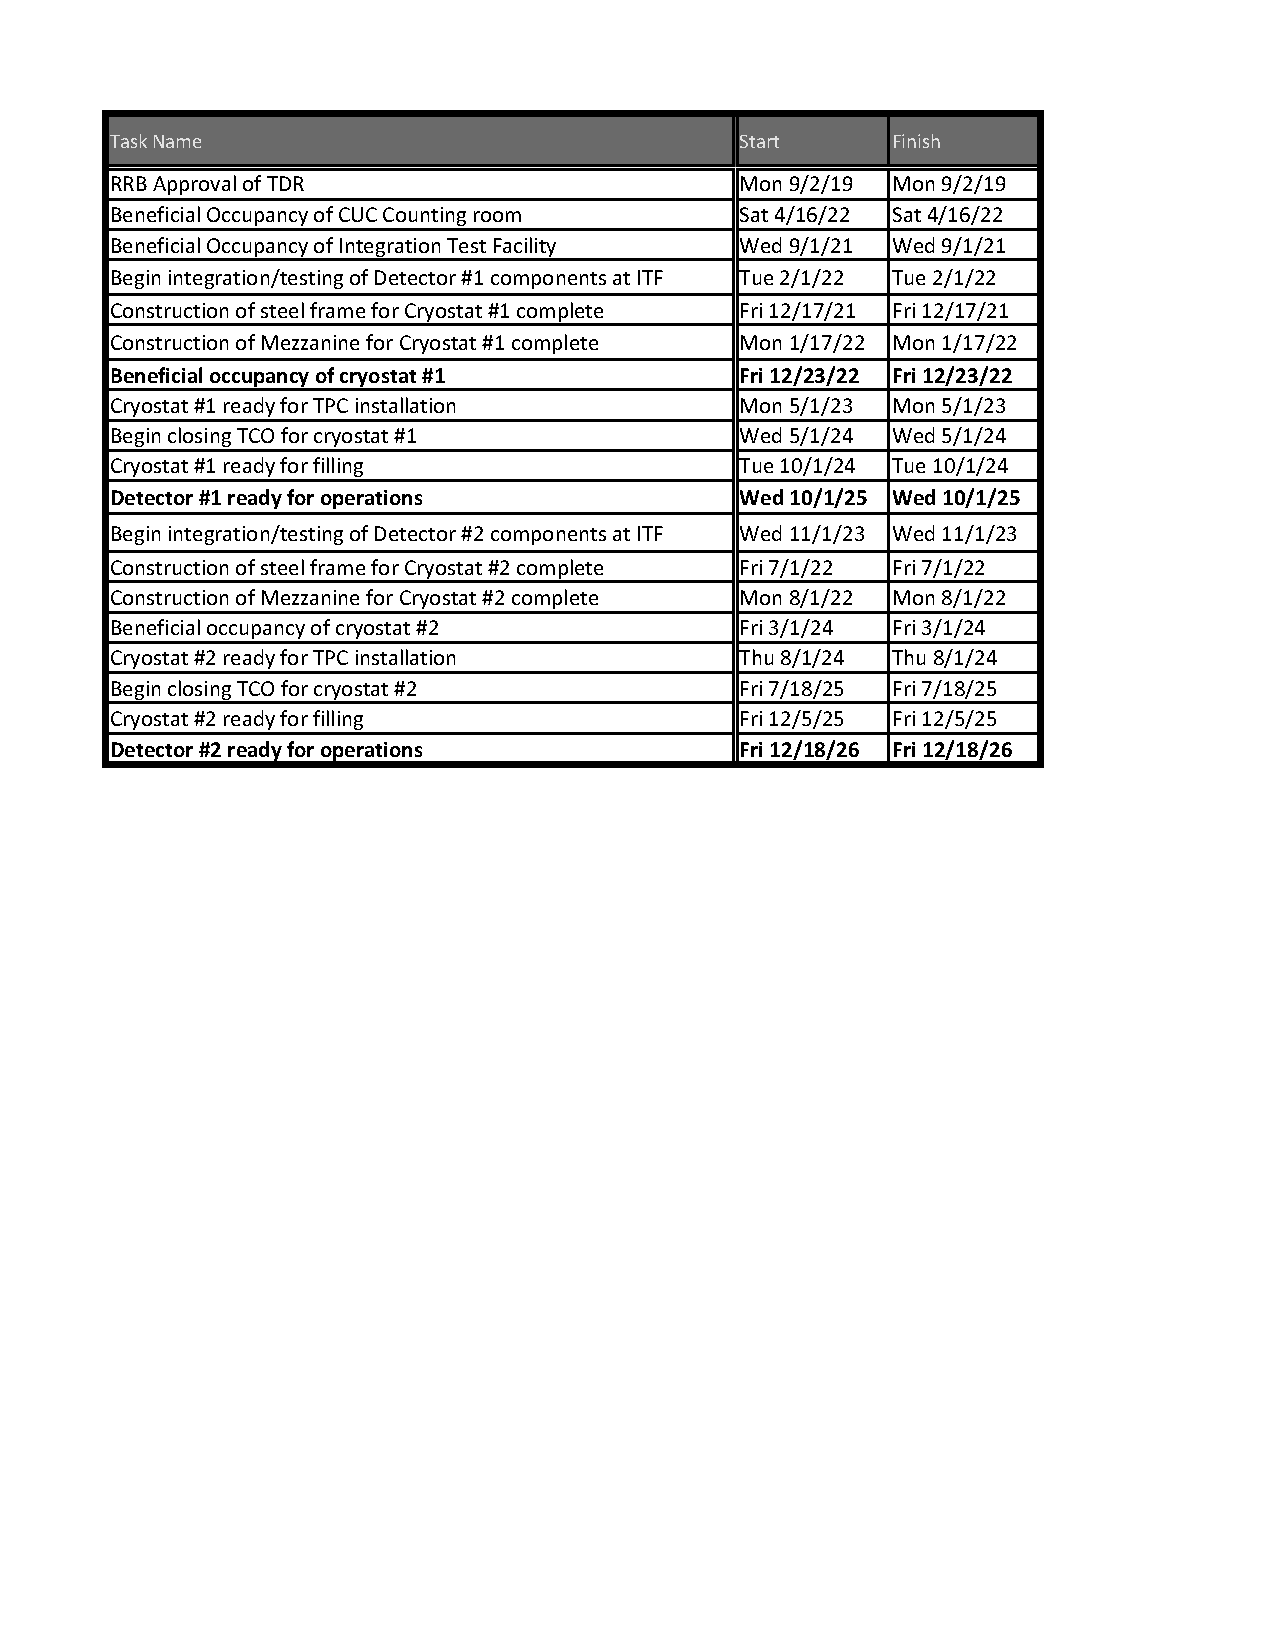
\includegraphics[width=\textwidth]{far-detector-generic/figures/FD_Cnst_Schedule}
    \caption{Overall \dword{dune} Project Tier-1 milestones.}
    \label{fig:DUNE_schedule}
  \end{center}
\end{figure}
\dword{tc} will maintain the IMS that links all consortia schedules
and contains appropriate milestones to monitor progress. The IMS
is envisioned to be maintained in MS-Project as it is expected
that many consortia will use this tool. It is currently envisioned as
three levels of control and notification milestones in addition to the
detailed consortia schedules. The highest level containing external
milestones, with the second level containing the key milestones for \dword{tc}
to monitor deliverables and installation progress, and the third level
containing the inter-consortia links. The schedules will go
under change control after agreement with each consortium on the
notification milestone dates and the TDR is approved.

In addition to the overall DUNE IMS for construction and
installation, a schedule of key consortia activity in the period
2018--19 leading up to the TDR has been developed.

In order to ensure that the \dword{dune} detector remains on schedule,
\dword{tc} will monitor schedule statusing from each consortium, will organize
reviews of schedules and risks as appropriate.  As schedule problems
arise \dword{tc} will work with the affected consortium to resolve the
problems. If problems cannot be solved, \dword{tc} will take the issue to the
TB and EB.

A monthly report with input from all consortia will be published by
\dword{tc}. This will include updates on consortia technical progress and
updates from \dword{tc} itself.


%%%%%%%%%%%%%%%%%%%%%%%%%%%%%%%%
\subsection{Risk}
\label{sec:fdsp-coord-risk}

The successful operation of \dword{protodune} will retire a great many
potential risks to \dword{dune}. This includes most risks associated with the
technical design, production processes, quality assurance, integration
and installation. Residual risks remain relating to design and
production modifications associated with scaling to \dword{dune}, mitigations
to known installation and performance issues in \dword{protodune}, underground
installation at SURF and organizational growth.

Some of the highest technical risks are: development of a system to
deliver 600~kV to the dual phase cathode, general delivery of the
required HV, cathode and field cage discharge to the cryostat
membrane, noise levels, particularly for the cold TPC electronics,
number of dead channels, lifetime of components surpassing 20 years,
quality control of all components, verification of improved LEM
performance, verification of new cold ADC and COLDATA performance,
argon purity, electron drift lifetime, photoelectron light yield,
incomplete calibration plan and incomplete connection of design to
physics. Other major risks include insufficient funding, optimistic
production schedules, incomplete integration, testing and installation
plans.

Key risks for \dword{tc} to manage include the following:
\begin{enumerate}
    \item Too much scope is unaccounted for by the consortia and falls
      to \dword{tc} and Common Fund.
    \item Insufficient organizational systems are put into place to
      ensure that this complex international mega-science project,
      including \dword{tc}, FNAL as Host Lab, SURF, DOE and all international
      partners continue to successfully work together to ensure
      appropriate rules and services are provided to enable success of
      the project.
  \item \dword{tc} is unable to obtain sufficient personnel resources so as to
    be able to ensure that \dword{tc} can oversee and coordinate all of its
    project tasks.  While the US has a special responsibility towards
    \dword{tc} as host country, it is expected that personnel resources will
    be directed to \dword{tc} from each collaborating country. Related to this
    risk is the fact that consortia deliverables are not really
    stand-alone subsystems; they are all parts of a single TPC. This
    elevates the requirements on coordination between consortia.
\end{enumerate}

The consortia have provided preliminary versions of risk analyses that
have been collected on the \dword{tc} webpage. These are being developed into
an overall risk register that will be monitored and maintained by \dword{tc}
in coordination with the consortia.

%%%%%%%%%%%%%%%%%%%%%%%%%%%%%%%%
\subsection{Reviews}
\label{sec:fdsp-coord-reviews}

\dword{tc} is responsible to review all stages of detector development
and works with each consortium to arrange reviews of the design
(\dword{pdr} and \dword{fdr}), production (\dword{prr} and
\dword{ppr}) and operational readiness (ORR) of their system.  These
reviews provide input for the TB to evaluate technical decisions.
Review reports are tracked by \dword{tc} and provide guidance as to
key issues that will require engineering oversight by the \dword{tc}
engineering team. \dword{tc} will maintain a calendar of \dword{dune}
reviews.

\dword{tc} will work with consortia leaders to review all detector designs,
with an expectation for a \dword{pdr}, followed by a \dword{fdr}.  All
major technology decisions will be reviewed prior to down-select.  \dword{tc}
may form task forces as necessary for specific issues that need more
in depth review.


Start of production of DUNE detector elements can commence only after
successful production readiness review. Regular production progress
reviews will be held once production has commenced. The \dwords{prr}
will typically include review of the production of ``Module 0'', the
first such module produced at the facility. \dword{tc} will work with
consortia leaders for all production reviews.

\dword{tc} is responsible to coordinate technical documents for the LBNC
Technical Design Review.

%%%%%%%%%%%%%%%%%%%%%%%%%%%%%%%%
\subsection{Quality Assurance}
\label{sec:fdsp-coord-qa}


The \dword{lbnf}/\dword{dune} \dword{qap} outlines the QA requirements
for all \dword{dune} consortia and describes how the requirements
shall be met. The consortia will be responsible for implementing a
quality plan that meet the requirements of the
\dword{lbnf}/\dword{dune} \dword{qap}.  The consortia implement the
plan through the development of individual quality plans, procedures,
guides, QC inspection and test requirements and travelers\footnote{The
  traveler is a document that details the fabrication and inspection
  steps and insures that all steps have been satisfactorily
  completed.}/test reports.  In lieu of a consortia specific quality
plan, the consortia may work under the \dword{lbnf}/\dword{dune}
\dword{qap} and develop Manufacturing/QC Plans, procedures and
documentation specific to their work scope.  The \dword{dune}
Technical Coordinator and consortia Leaders are responsible for
providing the resources needed to conduct the Project successfully,
including those required to manage, perform and verify work that
affects quality.  The \dword{dune} consortia Leaders are responsible
for identifying adequate resources to complete the work scope and to
ensure that their team members are adequately trained and qualified to
perform their assigned work.

The consortia work will be documented on travelers and applicable test
or inspection reports. Records of the fabrication, inspection and
testing will be maintained. When a component has been identified as
being in noncompliance to the design, the nonconforming condition
shall be documented, evaluated and dispositioned as use-as-is (does
not meet design but can meet functionality as is), rework (bring into
compliance with design), repair (will be brought into meeting
functionality but will not meet design) and scrap. For nonconforming
equipment or material that is dispositioned as use-as-is or repair, a
technical justification shall be provided allowing for the use of the
material or equipment and approved by the design authority.

The \dword{lbnf}/\dword{dune} \dword{qam} reports
to the \dword{lbnf} Project Manager and \dword{dune} Technical
Coordinator and provides oversight and support to the consortia
Leaders to ensure a consistent quality program.
\begin{enumerate}
  \item The \dword{qam} will plan reviews as independent assessments to assist
    the \dword{dune} Technical Coordinator in identifying opportunities for
    quality/performance-based improvement and to ensure compliance
    with specified requirements.
  \item The \dword{qam} is responsible to work with the consortia in
    developing their QA/QC Plans.
  \item The \dword{qam} will review consortia QA/QC activity, including
    production site visits.
  \item The \dword{qam} will participate in consortia Design Reviews, conduct
    Production Readiness Reviews prior to the start of production,
    conduct Production Progress Reviews on a regular basis (as
    described in Section~\ref{sec:fdsp-coord-reviews}), and perform
    follow-up visits to consortia facilities prior to shipment of
    components to ensure all components and documentation are
    satisfactory.
\item The \dword{qam} is responsible for performing assessments at the
  \dword{itf}, the Far Site and the Near Site to
  ensure the activities performed at these locations are in accordance
  with the \dword{lbnf}/\dword{dune} QA Program and applicable procedures,
  specifications and drawings.
\end{enumerate}

%%%%%%%%%%%%%%%%%%%%%%%%%%%%%%%%
\subsubsection{Document Control}
\label{sec:fdsp-coord-document}

\dword{tc} maintains repositories of project documents and drawings in two
document management systems.  DUNE Project documents will be stored in
the DUNE DocDB (\url{https://docs.dunescience.org}). DUNE drawings
will be stored in \dword{edms}
(\url{https://edms.cern.ch/ui/#!master/navigator/project?P:1637280201:1637280201:subDocs}).
\dword{tc} will maintain approved versions of QA, QC and testing plans,
installation plans, engineering and safety standards in the DUNE
DocDB.

Consortia have developed initial interface, risk, schedule and WBS
documents that will be put under change control and managed by the \dword{tc}
engineering team along with the consortia involved. These
are currently in DocDB and will likely go under change control later
in 2018, although they will continue to be developed through the TDR.

Thresholds for change control are described in the
\dword{lbnf}/\dword{dune} \dword{cmp}. The control process is further
described in Section~\ref{sec:fdsp-coord-integ-config}.

%%%%%%%%%%%%%%%%%%%%%%%%%%%%%%%%
\subsection{\dword{esh}}
\label{sec:fdsp-coord-esh}

The \dword{dune} \dword{esh} program is described in the
\dword{lbnf}/\dword{dune} \dword{ieshp}. This plan is maintained by
the \dword{lbnf}/\dword{dune} \dword{esh} Manager, who reports to the
\dword{lbnf} Project Manager and the Technical Coordinator. The
\dword{esh} manager is responsible to work with the consortia in
reviewing their hazards and their \dword{esh} plans.  The \dword{esh}
Manager is responsible to review \dword{esh} at production sites,
integration sites and at SURF. It is expected that the \dword{esh}
reviews will be conducted as part of the \dword{prr} and \dword{ppr}
process described in Section~\ref{sec:fdsp-coord-reviews}.
